\documentclass[margin=2mm]{standalone}
%\usepackage{bm}
%\usepackage{calligra}
\usepackage{amsmath} % assumes amsmath package installed
\usepackage{amssymb}  % assumes amsmath package installed
\newcommand{\setfont}[2]{{\fontfamily{#1}\selectfont #2}}
\usepackage{graphicx}
\usepackage{tikz}
\usetikzlibrary{3d}

\usetikzlibrary{calc}
\usetikzlibrary{patterns}
\usetikzlibrary{decorations.text}
\usetikzlibrary{decorations.pathmorphing}
\usetikzlibrary{decorations.markings}
\usetikzlibrary{arrows}
\usetikzlibrary{shapes}

%\pgfdeclareimage[width=2.0cm]{VectorFields}{EllipseBetaThird}
%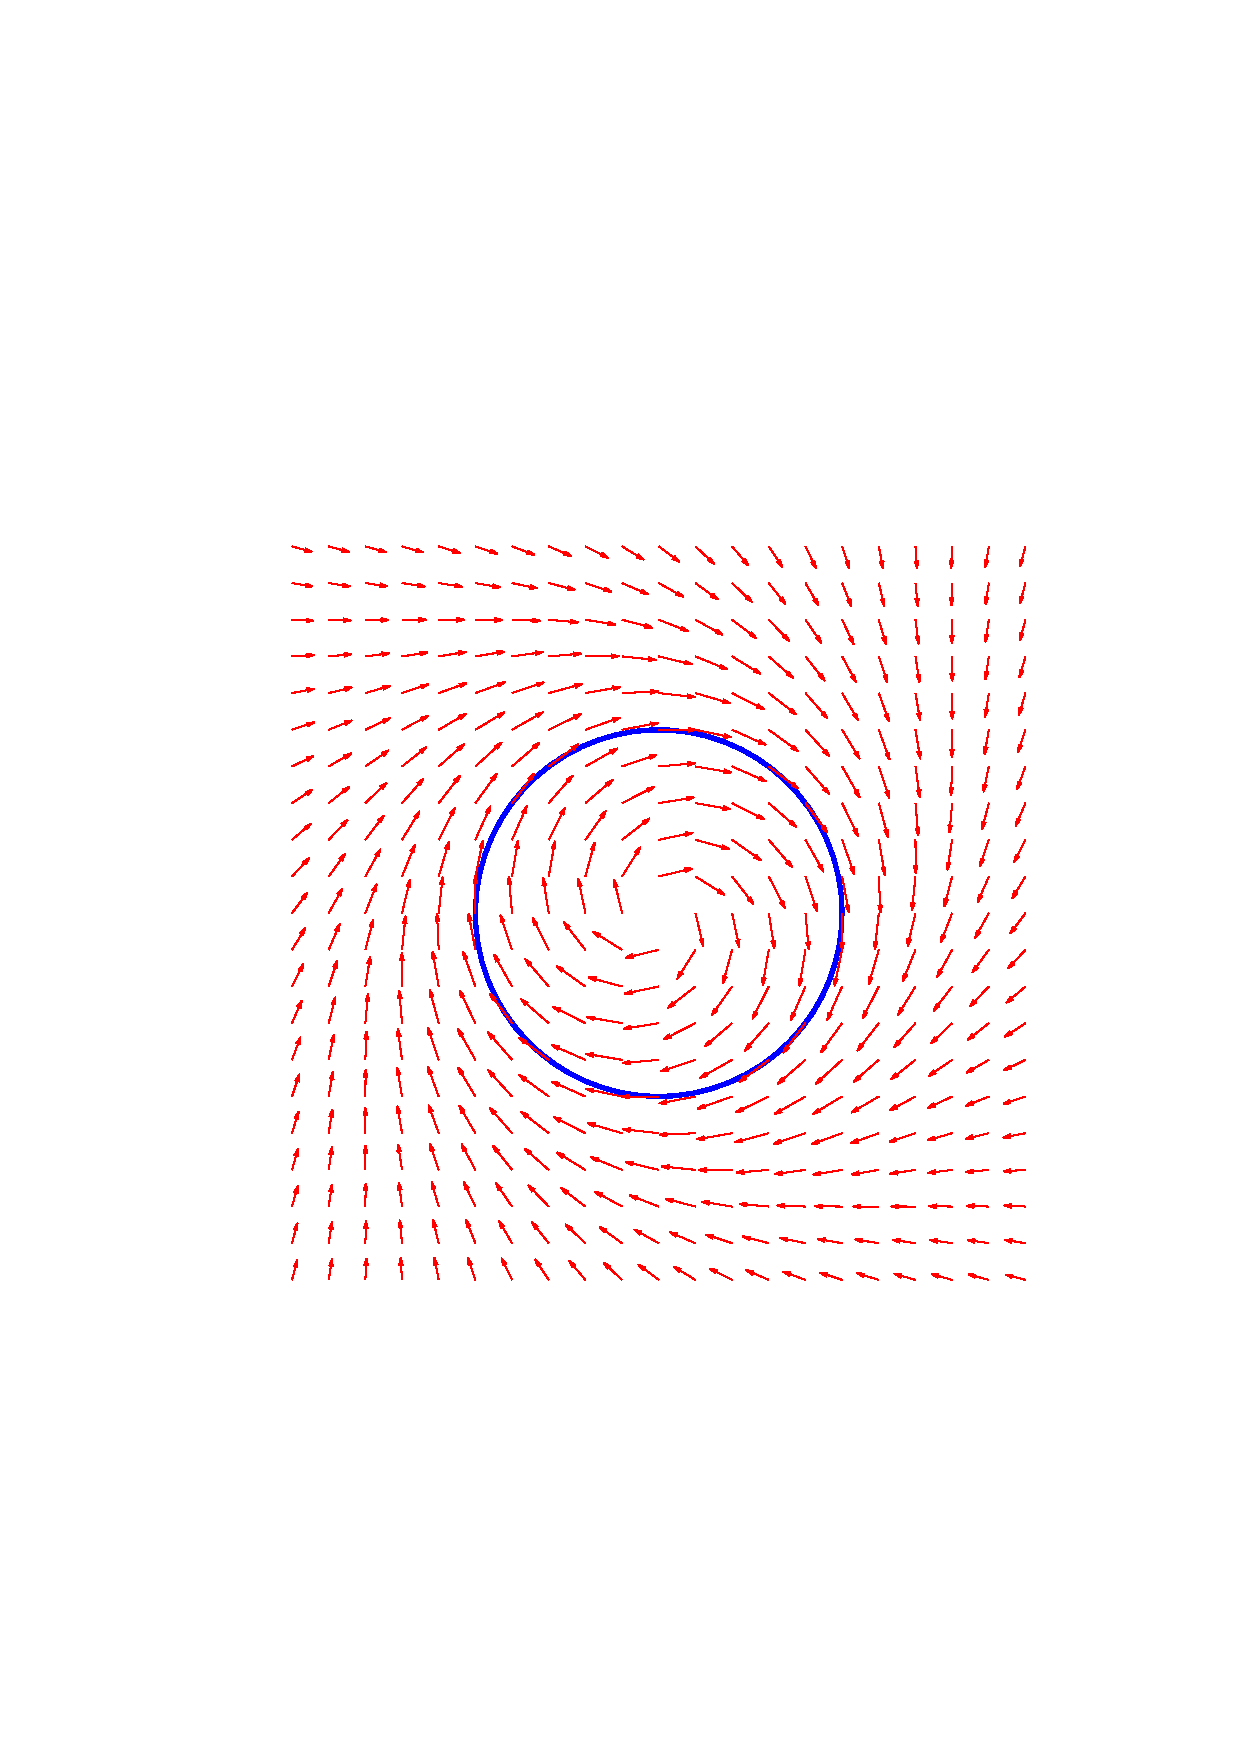
\includegraphics[trim=4cm 10cm 4cm 11cm, clip=true,keepaspectratio,width=0.45\linewidth]{../Fig3a_UnitCircle.pdf}

\newcommand{\picturefontsize}{\LARGE}
\newcommand{\pictureLineWidth}{0.8mm}

\begin{document}
% For every picture that defines or uses external nodes, you'll have to
% apply the 'remember picture' style. To avoid some typing, we'll apply
% the style to all pictures.
\tikzstyle{every picture}+=[remember picture]
\tikzstyle{na} = [baseline=-.5ex]

\begin{tikzpicture}

%\draw[help lines,thick] (-2,-4) grid (7,2);

\tikzstyle{vflabels}=[font=\tiny];
% First Line: Images


%\includegraphics[trim=1cm 7cm 0.5cm 7cm, clip=true,keepaspectratio,width=.5\linewidth]{./figures/Fig5a_DSshapesSymmetric}
%\includegraphics[trim=2cm 4.9cm 1.7cm 7cm, clip=true,keepaspectratio,width=.4\linewidth]{./figures/Fig5b_DSshapesZoomInSymmetric}

\node (imagea) at (0,0)
{\includegraphics[trim=1cm 7cm 0.5cm 7cm, clip=true,keepaspectratio,width=2cm]{../Fig5a_DSshapesSymmetric}}; 
\node[vflabels] at (0,-1.1) (labelimagea) {(a)};

\node (imageb) at (2.5,0.0)
{\includegraphics[trim=2cm 4.9cm 1.7cm 7cm, clip=true,keepaspectratio,width=2cm]{../Fig5b_DSshapesZoomInSymmetric}}; 
\node[vflabels] at (2.5,-1.1) (labelimageb) {(b)}; 


%\node (zero) at (0,0) {$(0,0)$};
\end{tikzpicture}
\end{document}
